\documentclass[11pt,a4paper]{report}

\usepackage[a4paper,margin=2.5cm]{geometry}
\usepackage{fontspec}
\usepackage[french]{babel}
\usepackage{microtype}
\usepackage{graphicx}
\usepackage{booktabs}
\usepackage{tabularx}
\usepackage{longtable}
\usepackage{array}
\usepackage{amsmath}
\usepackage{amssymb}
\usepackage{xcolor}
\usepackage{listings}
\usepackage{float}
\usepackage{pdflscape}
\usepackage{caption}
\usepackage[skip=\baselineskip,indent=1.5em]{parskip}
\usepackage{indentfirst}
\usepackage[numbers]{natbib}
\usepackage[hidelinks]{hyperref}

\graphicspath{{../}{../../}}
\newcolumntype{Y}{>{\raggedright\arraybackslash}X}
\newcolumntype{C}{>{\centering\arraybackslash}p{2.2cm}}
\renewcommand{\arraystretch}{1.18}

\lstdefinestyle{reportcode}{
  basicstyle=\ttfamily\small,
  columns=fullflexible,
  breaklines=true,
  frame=single,
  framerule=0.3pt,
  rulecolor=\color{black!25},
  backgroundcolor=\color{black!3}
}
\lstset{style=reportcode}

\title{\textbf{Fire Control System}\\
\large Modélisation fonctionnelle, réseau de Petri et vérification formelle}
\author{Paul Pitiot \and Maxime Crayssac \and Arthur Neuez}
\date{Année universitaire 2025--2026}

\begin{document}

\begin{titlepage}
  \centering
  \vspace*{1.2cm}
  
\includegraphics[width=0.32\textwidth]{cy-tech.png}\par
  \vspace{1.2cm}
  {\Huge\bfseries Fire Control System\par}
  \vspace{0.4cm}
  {\Large Modélisation fonctionnelle, réseau de Petri et vérification formelle\par}
  \vspace{1.5cm}
  {\large Rapport final du projet de programmation fonctionnelle\par}
  \vfill
  \begin{tabular}{rl}
    Étudiants : & Paul Pitiot \\
                & Maxime Crayssac \\
                & Arthur Neuez \\
    Technologie : & Scala, Akka Typed, Kafka, réseaux de Petri \\
    Dépôt : & \url{https://github.com/mcrayssac/Fire-Control-System}
  \end{tabular}
  \vfill
  {\large Année universitaire 2025--2026\par}
\end{titlepage}

\pagenumbering{roman}

\chapter*{Résumé}
\addcontentsline{toc}{chapter}{Résumé}
Ce rapport présente la conception et la validation d'un système de contrôle de tir modélisé comme un système critique concurrent. Le projet combine une implémentation distribuée en Scala avec Akka Typed, une représentation formelle par réseau de Petri et une vérification exhaustive des propriétés de sûreté et de vivacité. L'objectif n'est pas uniquement de simuler un cycle de tir nominal, mais de démontrer que les états dangereux sont inatteignables dans le modèle retenu : tir sans verrouillage, tir sans munition, tir sans autorisation, conflit entre tir et rechargement, stock négatif ou blocage global.

La démarche suit six axes : état de l'art, modélisation fonctionnelle, traduction vers un modèle formel, vérification des propriétés, comparaison entre modèle et implémentation, puis mode d'exécution interactif. La partie centrale du rapport est consacrée à la vérification formelle. Elle détaille l'exploration de l'espace d'états, les invariants structurels, les invariants métier, les propriétés LTL, la bornitude, la vivacité et l'absence de deadlock. Les résultats obtenus sont cohérents avec les objectifs de sûreté du projet : 111 marquages atteignables sont explorés, aucun deadlock n'est détecté, dix invariants métier et six propriétés temporelles sont satisfaits.

\tableofcontents
\listoffigures
\listoftables
\clearpage
\pagenumbering{arabic}

\chapter{Introduction}

\section{Contexte}
Un système de contrôle de tir (\emph{Fire Control System}, FCS) appartient à la famille des systèmes critiques : une action incorrecte peut entraîner des conséquences irréversibles. Il s'agit d'une chaîne de décision qui observe l'environnement, suit une cible, vérifie la disponibilité des ressources, demande une autorisation, puis déclenche ou refuse l'action de tir. Chaque étape porte donc une responsabilité de sûreté : une information absente, incohérente ou traitée trop tôt peut modifier radicalement la décision finale.

La gravité d'un tel système vient du fait qu'un défaut logiciel ne se limite pas à une erreur d'affichage ou à un résultat numérique imprécis. Dans un FCS, une transition mal contrôlée peut conduire à un tir sans cible verrouillée, sans munition cohérente, sans autorisation explicite, pendant une phase de rechargement ou sans journalisation exploitable. Ces situations doivent être impossibles par construction, et non simplement rares dans les tests.

Un exemple concret est celui d'un char qui détecte un véhicule blindé adverse et prépare un tir avec une munition de type \texttt{APFSDS}. Dans l'implémentation, le cycle doit vérifier que la cible est suivie avec une confiance suffisante, que la munition demandée est disponible, que les règles d'engagement autorisent le tir, puis seulement déclencher l'action. Le code distingue plusieurs types de munitions, notamment \texttt{APFSDS}, \texttt{HEAT}, \texttt{HESH} et \texttt{HE}. Le réseau de Petri les abstrait ensuite en un stock borné générique, car la propriété de sûreté étudiée est la disponibilité et la synchronisation de la munition, non la physique détaillée de chaque obus.

Le projet reste une abstraction académique : il ne modélise ni un calcul balistique réel complet, ni une doctrine opérationnelle exhaustive. En revanche, il reprend la discipline des systèmes critiques : comportement \emph{fail-safe}, préconditions explicites, traçabilité des événements et raisonnement exhaustif sur les états atteignables. La sûreté du logiciel ne peut donc pas être ramenée à quelques scénarios de test. Le système doit empêcher par construction les situations dangereuses, notamment un tir sans cible verrouillée, sans munition disponible ou sans autorisation.

Le projet étudié adopte une double approche. D'une part, le comportement opérationnel est réalisé avec le modèle d'acteurs Akka Typed, qui permet de représenter naturellement la concurrence entre capteur, suivi balistique, gestion des munitions, commande et supervision. D'autre part, les comportements critiques sont abstraits dans un réseau de Petri fini afin de permettre une exploration exhaustive de l'espace d'états.

\section{Objectifs et méthode}
Les objectifs du projet sont couverts par six livrables techniques : un état de l'art, un modèle Akka fonctionnel, une traduction vers un réseau de Petri, une vérification de propriétés, une simulation comparée entre réel et formel, et un mode interactif. Le fil conducteur du rapport est la traçabilité entre ces livrables : chaque composant implémenté est relié à une place, une transition ou une propriété du modèle formel.

La méthode de validation est la suivante :
\begin{enumerate}
  \item concevoir une architecture fonctionnelle concurrente ;
  \item identifier les états et transitions critiques ;
  \item construire un réseau de Petri fini ;
  \item explorer l'ensemble des marquages atteignables ;
  \item vérifier des invariants de sûreté et des propriétés LTL ;
  \item comparer les traces produites par le modèle formel et l'implémentation Akka.
\end{enumerate}

\chapter{État de l'art}

\section{Vérification formelle}
La vérification formelle consiste à prouver mathématiquement qu'un système respecte certaines propriétés. Contrairement au test logiciel, qui observe un nombre fini de scénarios, elle raisonne sur l'ensemble des comportements représentés par un modèle. Cette approche est particulièrement adaptée aux domaines critiques comme l'avionique, le nucléaire ou les systèmes militaires. L'échec du vol 501 d'Ariane 5, causé par un dépassement d'entier non détecté, illustre la nécessité d'une analyse systématique des comportements logiciels \citep{lions1996}.

Deux familles d'approches dominent. Le \emph{model checking} explore automatiquement un modèle fini et fournit des contre-exemples en cas de violation. Le \emph{theorem proving} permet de raisonner sur des espaces plus généraux, mais demande une expertise logique plus importante et davantage d'intervention humaine \citep{clarke1999,baier2008}. Le FCS étudié ici se prête au \emph{model checking} : son réseau de Petri produit 111 marquages atteignables, ce qui rend possible une exploration exhaustive.

\section{Réseaux de Petri}
Avant d'introduire l'écriture mathématique, il faut lire un réseau de Petri comme une carte des situations possibles du système. Les \emph{places} sont les états ou ressources observables, par exemple être au repos, avoir une cible verrouillée ou posséder des munitions. Les \emph{transitions} sont les actions autorisées qui font évoluer le système. Les \emph{jetons} indiquent ce qui est vrai à un instant donné : un jeton dans une place de contrôle signifie que cette phase est active ; plusieurs jetons dans une place ressource représentent une quantité disponible.

Un réseau de Petri est alors résumé par le quintuplet :
\[
N = (P, T, Pre, Post, M_0)
\]
où $P$ est l'ensemble des places, $T$ l'ensemble des transitions, $Pre$ et $Post$ décrivent les arcs entrants et sortants, et $M_0$ est le marquage initial \citep{murata1989,peterson1981}. Les jetons portés par les places représentent l'état courant. Une transition $t$ est franchissable dans un marquage $M$ si toutes ses préconditions sont satisfaites :
\[
\forall p \in P,\quad M(p) \geq Pre(t,p)
\]
Cette condition signifie simplement qu'une action ne peut être exécutée que si chaque place nécessaire contient assez de jetons. Dans notre projet, cela revient par exemple à dire qu'un tir ne peut pas passer la synchronisation si l'autorisation ou la munition chargée manque.

Son franchissement produit alors le nouveau marquage :
\[
M'(p) = M(p) - Pre(t,p) + Post(t,p)
\]
On retire les jetons consommés par l'action, puis on ajoute ceux produits après l'action. Cette règle est la version formelle d'un changement d'état : quitter l'état \emph{Ready\_To\_Fire}, entrer dans l'état \emph{Firing}, et ajouter un événement dans la file Kafka.

La matrice d'incidence $C = Post - Pre$ résume l'effet net des transitions. Elle permet d'exprimer les propriétés structurelles du réseau, notamment les P-invariants et les T-invariants. Dans ce projet, le réseau de Petri sert à représenter les états critiques du cycle de tir, les ressources finies et les synchronisations entre conditions.

\section{Logique temporelle linéaire}
La logique temporelle linéaire (LTL) permet d'exprimer des propriétés sur les traces d'exécution \citep{pnueli1977}. Une trace est la suite des états traversés par le système. LTL sert donc à traduire des phrases comme ``le tir et le rechargement ne se superposent jamais'' ou ``après une erreur, on doit pouvoir revenir au repos''.

Elle complète les invariants statiques en décrivant l'évolution attendue du système. Les opérateurs utilisés sont :

\begin{table}[H]
\centering
\caption{Opérateurs LTL utilisés}
\begin{tabularx}{\textwidth}{lclY}
\toprule
Opérateur & Symbole & Type & Signification \\
\midrule
Globally & $G(\varphi)$ & sûreté & $\varphi$ est vraie dans tous les états futurs. \\
Finally & $F(\varphi)$ & vivacité & $\varphi$ sera vraie dans au moins un état futur. \\
Next & $X(\varphi)$ & pas suivant & $\varphi$ est vraie dans l'état immédiatement suivant. \\
Until & $\varphi\,U\,\psi$ & évolution & $\varphi$ reste vraie jusqu'à ce que $\psi$ devienne vraie. \\
\bottomrule
\end{tabularx}
\end{table}

Les propriétés de sûreté affirment qu'un mauvais état n'arrive jamais ; les propriétés de vivacité affirment qu'un bon état finit par arriver. Pour un système de tir, les deux dimensions sont indispensables : il faut interdire les combinaisons dangereuses, mais aussi garantir la récupération après erreur et le retour à un état contrôlable.

\section{Modèle d'acteurs}
Le modèle d'acteurs représente la concurrence par des entités autonomes qui possèdent leur propre état et communiquent par messages asynchrones \citep{hewitt1973,agha1986}. Akka Typed fournit une implémentation Scala de ce modèle avec typage des messages, supervision hiérarchique et isolation des états \citep{akka2024}. La correspondance avec les réseaux de Petri est naturelle : un état d'acteur peut être abstrait par une place, la réception d'un message par une transition, et une synchronisation par une transition à plusieurs préconditions.

\chapter{Architecture fonctionnelle du FCS}

\section{Choix d'architecture}
Le FCS réunit les caractéristiques d'un système critique distribué : concurrence entre sous-systèmes, synchronisation stricte avant tir, ressources finies et tolérance aux erreurs. L'architecture Akka Typed répond à ces contraintes en isolant les responsabilités dans des acteurs typés. Chaque acteur ne traite qu'un message à la fois, ce qui évite les accès concurrents directs à un état partagé.

\section{Acteurs}
L'implémentation repose sur huit acteurs organisés autour d'un superviseur racine :

La représentation suivante est un arbre de responsabilité. Chaque ligne est un acteur Akka ; l'indentation indique que le \texttt{SupervisorActor} crée et surveille les acteurs enfants. L'objectif est d'éviter un état partagé global : chaque acteur possède son état et communique par messages.

\begin{lstlisting}
SupervisorActor
|-- SensorActor
|-- TrackingActor
|-- AmmoActor
|-- CommandActor
|-- FireControlActor
|-- KafkaProducerActor
+-- KafkaConsumerActor
\end{lstlisting}

\begin{table}[H]
\centering
\caption{Responsabilités des acteurs Akka}
\begin{tabularx}{\textwidth}{lY}
\toprule
Acteur & Responsabilité \\
\midrule
SupervisorActor & Création, supervision et redémarrage des acteurs enfants. \\
SensorActor & Détection des cibles et déclenchement du cycle. \\
TrackingActor & Calcul balistique, verrouillage et confiance de suivi. \\
AmmoActor & Gestion du stock et chargement des munitions. \\
CommandActor & Validation des règles d'engagement. \\
FireControlActor & Orchestration du cycle, synchronisation des confirmations, tir, rechargement et refroidissement. \\
KafkaProducerActor & Publication des événements opérationnels. \\
KafkaConsumerActor & Collecte de l'audit trail. \\
\bottomrule
\end{tabularx}
\end{table}

\section{Cycle nominal}
Le cycle nominal part d'une détection de cible. Le FireControlActor déclenche ensuite trois activités : verrouillage balistique, chargement d'une munition et demande d'autorisation. Le tir n'est exécuté que lorsque les trois confirmations sont reçues :

La formule suivante condense notre choix de conception : le booléen \texttt{readyToFire} ne vaut vrai que si les trois verrous métier sont levés. Le symbole $\land$ signifie ``et logique'' ; aucune des trois conditions ne peut remplacer les deux autres.
\[
readyToFire = targetLocked \land ammoLoaded \land fireAuthorized
\]
Cette condition correspond directement à la transition de synchronisation $T4$ du réseau de Petri.

La trace ci-dessous vulgarise le même cycle sous forme de messages. Chaque flèche représente une demande, une confirmation ou un changement de phase observé dans l'application.

\begin{lstlisting}
Detection -> Tracking -> TargetLockConfirmed
          -> AmmoActor -> AmmoLoadConfirmed
          -> CommandActor -> FireAuthConfirmed
          -> readyToFire -> FireExecuted
          -> ReloadTimeout -> CooldownTimeout -> Idle
\end{lstlisting}

\section{Gestion des erreurs et journalisation}
Les principaux cas d'erreur sont le refus de verrouillage, le refus d'autorisation, l'absence de munition et l'erreur système. Chaque situation produit une réponse contrôlée : abandon du cycle ou redémarrage supervisé. Les événements sont publiés sur des topics Kafka dédiés, ce qui assure une trace exploitable des actions critiques.

\begin{table}[H]
\centering
\caption{Situations d'erreur prises en charge}
\begin{tabularx}{\textwidth}{lY}
\toprule
Situation & Comportement \\
\midrule
Échec de verrouillage & Le TrackingActor signale un échec et le cycle est abandonné. \\
Refus d'autorisation & Le CommandActor refuse le tir si les règles d'engagement ne sont pas satisfaites. \\
Stock épuisé & L'AmmoActor signale l'impossibilité de charger une munition. \\
Erreur système & Le SupervisorActor applique une stratégie de récupération. \\
\bottomrule
\end{tabularx}
\end{table}

\chapter{Modèle formel par réseau de Petri}

\section{Définition du modèle}
Dans le modèle final, chaque place est nommée $P0$, $P1$, etc. pour rester compacte dans les formules. Chaque transition est nommée $T0$, $T1$, etc. pour identifier une action franchissable. Cette numérotation n'est pas arbitraire : elle sert de pont entre le diagramme, le code Scala et les résultats de vérification.

Le réseau de Petri du FCS contient 13 places et 12 transitions :
\[
|P| = 13,\quad |T| = 12
\]
Le symbole $|P|$ signifie ``nombre de places'' et $|T|$ signifie ``nombre de transitions''. Le marquage initial décrit ensuite la photographie du système au démarrage, dans l'ordre des places $P0$ à $P12$ :
\[
M_0 = (1,0,0,0,0,0,0,0,0,0,n,0,0)
\]
où $n$ représente le stock initial de munitions. Le jeton placé dans $P0$ indique que le système démarre au repos.

Le tableau des places se lit comme un dictionnaire. Les places de type contrôle décrivent une phase du cycle ; les places de type ressource comptent une quantité qui peut augmenter ou diminuer.

\begin{table}[H]
\centering
\caption{Places du réseau de Petri}
\begin{tabularx}{\textwidth}{cllY}
\toprule
Place & Nom & Type & Rôle \\
\midrule
P0 & Idle & contrôle & Système au repos. \\
P1 & Target\_Detected & contrôle & Cible détectée. \\
P2 & Target\_Locked & contrôle & Verrouillage confirmé. \\
P3 & Ammo\_Loaded & contrôle & Munition chargée. \\
P4 & Fire\_Authorized & contrôle & Autorisation accordée. \\
P5 & Ready\_To\_Fire & contrôle & Préconditions réunies. \\
P6 & Firing & contrôle & Tir en cours. \\
P7 & Reloading & contrôle & Rechargement. \\
P8 & Cooldown & contrôle & Refroidissement. \\
P9 & Error\_State & contrôle & Erreur détectée. \\
P10 & Ammo\_Stock & ressource & Stock de munitions. \\
P11 & Kafka\_Queue & ressource & Événements en attente. \\
P12 & Log\_Recorded & ressource & Événements journalisés. \\
\bottomrule
\end{tabularx}
\end{table}

Le tableau des transitions décrit les actions autorisées. La partie gauche de la flèche contient les places qui doivent posséder un jeton avant l'action ; la partie droite contient les places qui recevront un jeton après l'action.

\begin{table}[H]
\centering
\caption{Transitions du réseau de Petri}
\begin{tabularx}{\textwidth}{clY}
\toprule
Transition & Nom & Préconditions et postconditions \\
\midrule
T0 & detect\_target & $\{P0,P10\} \rightarrow \{P1,P10,P11\}$ \\
T1 & lock\_target & $\{P1\} \rightarrow \{P2\}$ \\
T2 & load\_ammo & $\{P10\} \rightarrow \{P3\}$ \\
T3 & authorize\_fire & $\{P2\} \rightarrow \{P4\}$ \\
T4 & ready\_sync & $\{P3,P4\} \rightarrow \{P5\}$ \\
T5 & fire & $\{P5\} \rightarrow \{P6,P11\}$ \\
T6 & end\_fire & $\{P6\} \rightarrow \{P7\}$ \\
T7 & reload\_complete & $\{P7\} \rightarrow \{P8\}$ \\
T8 & cooldown\_complete & $\{P8\} \rightarrow \{P0\}$ \\
T9 & error\_detected & $\{P0\} \rightarrow \{P9\}$ \\
T10 & error\_recovery & $\{P9\} \rightarrow \{P0\}$ \\
T11 & kafka\_log & $\{P11\} \rightarrow \{P12\}$ \\
\bottomrule
\end{tabularx}
\end{table}

La figure donne une lecture visuelle du même modèle : les cercles sont les places, les rectangles sont les transitions, les flèches sont les préconditions et postconditions, et les jetons matérialisent l'état courant.

\begin{figure}[H]
\centering
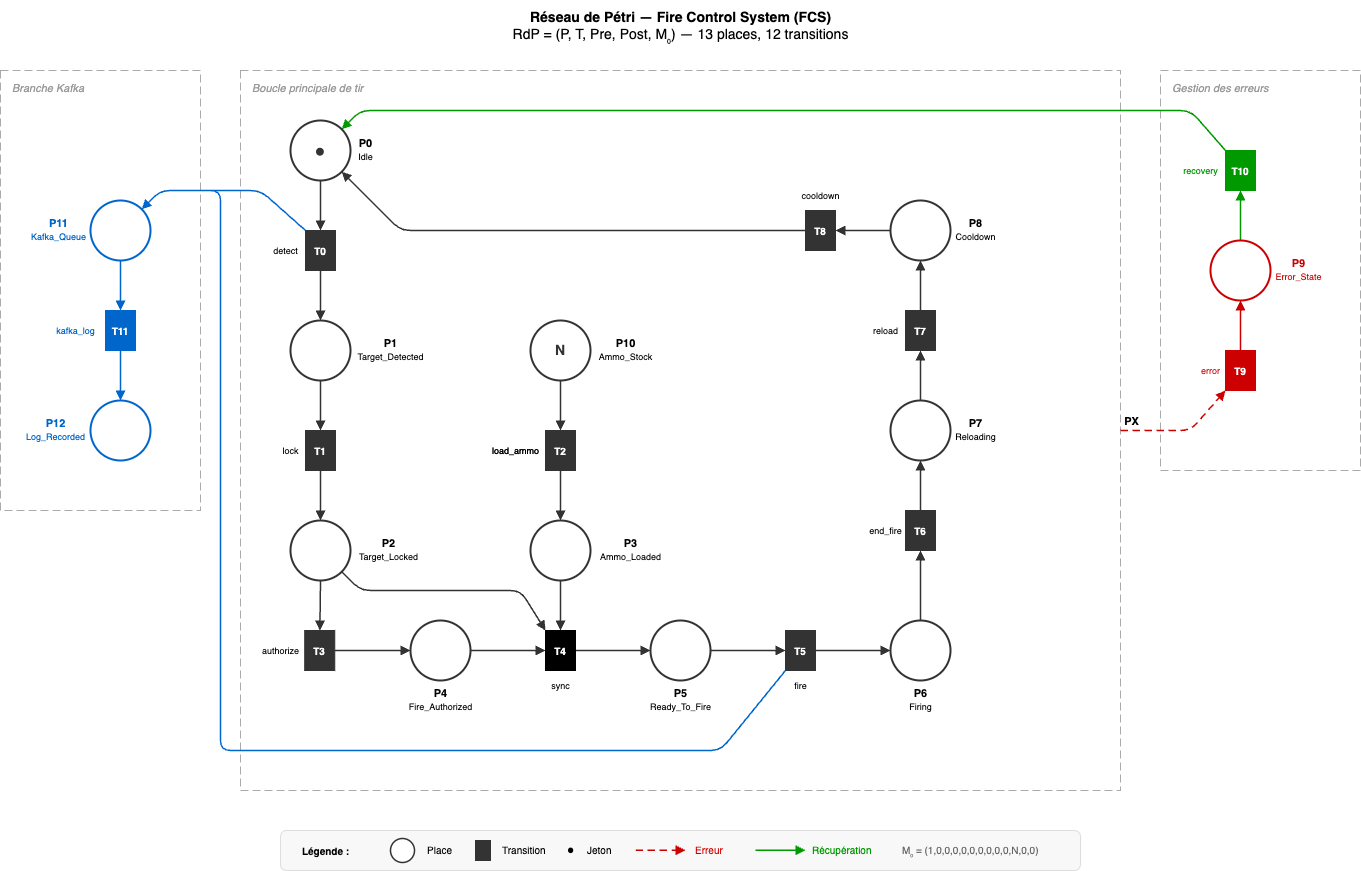
\includegraphics[width=\textwidth]{fcs_petri_net.drawio.png}
\caption{Réseau de Petri du Fire Control System}
\label{fig:petri-net}
\end{figure}

\section{Correspondance avec Akka}
La traduction formelle conserve les responsabilités critiques des acteurs. Le SensorActor correspond à la détection, le TrackingActor au verrouillage, l'AmmoActor au chargement, le CommandActor à l'autorisation, le FireControlActor à la synchronisation et au cycle de tir, et le SupervisorActor au cycle d'erreur/récupération.

Le tableau suivant explicite cette traduction. Il ne cherche pas à recopier tout le code Akka ; il garde uniquement les états et actions qui ont un impact direct sur la sûreté du tir.

\begin{table}[H]
\centering
\caption{Correspondance entre acteurs et réseau de Petri}
\begin{tabularx}{\textwidth}{lYY}
\toprule
Acteur Akka & Places & Transitions \\
\midrule
SensorActor & P0, P1 & T0 \\
TrackingActor & P1, P2 & T1 \\
AmmoActor & P10, P3 & T2 \\
CommandActor & P2, P4 & T3 \\
FireControlActor & P3 à P8 puis P0 & T4 à T8 \\
SupervisorActor & P0, P9 & T9, T10 \\
KafkaProducerActor & P11, P12 & T11 \\
\bottomrule
\end{tabularx}
\end{table}

\section{Hypothèses d'abstraction}
Le modèle formel abstrait les types précis de munitions, les calculs balistiques détaillés, les délais réels et les politiques internes de supervision. Ces choix réduisent la complexité sans supprimer les conditions de sûreté essentielles. Le modèle conserve ce qui influence directement la validité d'un tir : disponibilité d'une munition, verrouillage, autorisation, état de tir, rechargement, refroidissement, erreurs et journalisation.

\chapter{Vérification formelle}
\label{chap:verification}

\section{Objectif de la vérification}
Cette partie constitue le cœur du rapport. L'objectif est de démontrer que le modèle formel ne permet pas d'atteindre des états dangereux et que les comportements attendus restent possibles. La vérification est donc organisée autour de trois niveaux complémentaires :
\begin{itemize}
  \item l'exploration exhaustive des marquages atteignables ;
  \item les invariants, qui expriment des propriétés vraies dans tous les états ;
  \item les propriétés LTL, qui expriment des contraintes sur l'évolution des traces.
\end{itemize}

Les tests classiques valident quelques scénarios représentatifs. La vérification formelle apporte une garantie plus forte : tous les marquages atteignables depuis $M_0$ sont analysés. Dans le contexte d'un système de contrôle de tir, cette exhaustivité est indispensable, car un seul état dangereux suffit à invalider le modèle.

\section{Pipeline de vérification}
Le pipeline appliqué au projet part du réseau de Petri construit dans le code Scala, puis explore son espace d'états avant de vérifier les propriétés.

Le schéma ci-dessous se lit de gauche à droite. Chaque bloc transforme le modèle en une information plus exploitable : d'abord le réseau, puis tous ses états possibles, puis les propriétés vérifiées, enfin la comparaison avec l'exécution Akka.

\begin{figure}[H]
\centering
\begin{tabularx}{0.96\textwidth}{>{\centering\arraybackslash}X>{\centering\arraybackslash}X>{\centering\arraybackslash}X>{\centering\arraybackslash}X}
\fbox{\parbox{0.18\textwidth}{\centering Construction\\du réseau}} &
\fbox{\parbox{0.18\textwidth}{\centering Exploration\\BFS}} &
\fbox{\parbox{0.18\textwidth}{\centering Invariants\\et LTL}} &
\fbox{\parbox{0.18\textwidth}{\centering Comparaison\\Akka}} \\
\end{tabularx}
\caption{Chaîne de vérification du FCS}
\label{fig:pipeline-verification}
\end{figure}

La première étape produit les places, transitions, préconditions, postconditions et le marquage initial. La deuxième étape énumère les marquages atteignables par parcours en largeur. La troisième étape applique les propriétés de sûreté, de vivacité et de conservation. La dernière étape compare les traces attendues du réseau de Petri aux événements observés dans l'implémentation Akka.

\section{Exploration de l'espace d'états}
L'exploration exhaustive est effectuée par BFS avec un stock initial de trois munitions. BFS signifie \emph{Breadth-First Search}, ou parcours en largeur : l'algorithme part de $M_0$, franchit toutes les transitions possibles, puis recommence depuis chaque nouvel état découvert. Chaque nœud du graphe représente un marquage et chaque arc correspond au franchissement d'une transition.

Le tableau suivant résume donc la taille réelle du comportement étudié. Les 111 marquages sont les états effectivement atteignables, et non les états imaginés ou testés manuellement.

\begin{table}[H]
\centering
\caption{Résultats de l'exploration exhaustive}
\begin{tabularx}{0.7\textwidth}{YC}
\toprule
Métrique & Valeur \\
\midrule
Marquages atteignables & \textbf{111} \\
Arcs du graphe d'accessibilité & \textbf{227} \\
Deadlocks détectés & \textbf{0} \\
\bottomrule
\end{tabularx}
\end{table}

Le nombre de marquages reste suffisamment faible pour permettre une analyse complète. L'absence de deadlock signifie qu'aucun marquage atteignable ne bloque totalement le système. Cette propriété est importante : un FCS ne doit pas rester dans un état sans issue, notamment après erreur, rechargement ou refroidissement.

\section{Invariants structurels}
Les P-invariants expriment des lois de conservation. On peut les lire comme des compteurs pondérés qui doivent garder la même valeur, quel que soit le chemin pris dans le réseau. Le vecteur $y$ indique quelles places participent au compteur et avec quel poids.

Un vecteur $y$ est un P-invariant si :
\[
C^T y = 0
\]
Ici $C^T$ est la matrice d'incidence transposée : elle permet de vérifier que les gains et pertes de jetons s'annulent pour ce compteur. Dans ce cas, la quantité $y^T M$ reste constante pour tout marquage atteignable $M$. Ces invariants ne dépendent pas d'un scénario particulier ; ils décrivent la structure même du réseau.

Le premier invariant trouvé est le vecteur suivant. Les valeurs à 1 désignent les places prises dans le compteur ; les valeurs à 0 désignent celles qui sont ignorées :
\[
y_1 = (1,1,1,0,1,1,1,1,1,1,0,0,0)
\]
Il représente la conservation du flux de contrôle :
\[
P0 + P1 + P2 + P4 + P5 + P6 + P7 + P8 + P9 = 1
\]
Il garantit que le système possède exactement un état principal actif parmi les places de contrôle retenues. Cette propriété empêche les combinaisons incohérentes où le système serait simultanément au repos, en tir, en rechargement ou en erreur.

Le second invariant utilise des poids différents selon les places. Les coefficients 2 indiquent que certaines ressources ou phases comptent double dans la conservation globale :
\[
y_2 = (1,0,0,2,0,2,1,1,1,1,2,1,1)
\]
Il relie les places de contrôle et les places ressource. Il montre que les consommations et productions de jetons sont cohérentes avec la conservation globale attendue du modèle. Les deux invariants sont vérifiés sur les 111 marquages atteignables.

\section{Invariants métier}
Les invariants métier traduisent les exigences de sûreté du FCS. Ils ne se limitent pas à des propriétés mathématiques abstraites : chaque invariant correspond à une interdiction ou obligation opérationnelle.

Le tableau doit être lu comme un contrat entre le modèle et le projet. La colonne informelle exprime l'idée métier ; la colonne formelle indique comment cette idée est vérifiée sur les marquages ou transitions.

\begin{longtable}{p{1.2cm}p{4cm}p{6.2cm}p{1.8cm}}
\caption{Invariants métier vérifiés}
\label{tab:business-invariants}\\
\toprule
ID & Exigence informelle & Interprétation formelle & Résultat \\
\midrule
\endfirsthead
\toprule
ID & Exigence informelle & Interprétation formelle & Résultat \\
\midrule
\endhead
INV1 & Pas de tir sans verrouillage & La synchronisation $T4$ dépend de $P4$, produit uniquement après verrouillage et autorisation. & OK \\
INV2 & Pas de tir sans munition chargée & $T4$ exige $P3$, produit par $T2$ après consommation d'une munition disponible. & OK \\
INV3 & Pas de tir sans autorisation & $T4$ exige $P4$, produit par $T3$ après validation de commande. & OK \\
INV4 & Stock non négatif & Pour tout marquage $M$, $M(P10) \geq 0$. & OK \\
INV5 & Exclusion tir/rechargement & Pour tout marquage $M$, $M(P6)+M(P7)\leq 1$. & OK \\
INV6 & Pas de tir pendant refroidissement & $M(P6)>0 \Rightarrow M(P8)=0$. & OK \\
INV7 & Conservation du flux de contrôle & La somme des places de contrôle principales reste égale à 1. & OK \\
INV8 & Tout tir est journalisé & Si le tir est atteint, un événement de journalisation devient atteignable. & OK \\
INV9 & Retour à l'état idle & Des états avec $M(P0)>0$ restent atteignables après les cycles. & OK \\
INV10 & Absence de deadlock & Aucun marquage atteignable n'est sans transition franchissable. & OK \\
\bottomrule
\end{longtable}

Les invariants INV1, INV2 et INV3 forment le noyau de sûreté du tir : ils empêchent toute exécution de $T5$ si les préconditions opérationnelles n'ont pas été réunies. INV5 et INV6 empêchent les recouvrements dangereux entre phases incompatibles. INV4 protège la ressource finie, tandis qu'INV8 assure la traçabilité. INV10 élargit la sûreté à l'ensemble du cycle en garantissant qu'aucun état atteignable ne piège définitivement le système.

\section{Propriétés LTL}
Les invariants décrivent des états ; les propriétés LTL décrivent des traces. Cette distinction est essentielle. Un invariant peut prouver qu'un état interdit n'est jamais atteint, mais il ne suffit pas toujours à prouver qu'une action attendue finit par se produire.

Dans les formules ci-dessous, $G$ signifie ``toujours'', $F$ signifie ``finalement'', $\neg$ signifie ``non'', $\land$ signifie ``et'', et $\rightarrow$ signifie ``implique''. Les noms comme \emph{firing}, \emph{reloading} ou \emph{idle} sont des prédicats : ils valent vrai lorsque le marquage contient un jeton dans la place correspondante. Les formules LTL utilisées combinent donc sûreté, vivacité, récupération et traçabilité.

\begin{table}[H]
\centering
\caption{Propriétés LTL vérifiées}
\small
\begin{tabularx}{\textwidth}{p{0.6cm}p{3.4cm}p{2.4cm}Yp{1.6cm}}
\toprule
\# & Formule & Type & Signification & Résultat \\
\midrule
1 & $G(\neg(firing \land reloading))$ & Sûreté & Le tir et le rechargement ne sont jamais actifs simultanément. & OK \\
2 & $G(fire \rightarrow F(log\_recorded))$ & Traçabilité & Chaque tir finit par produire une trace journalisée. & OK \\
3 & $G(error \rightarrow F(idle))$ & Récupération & Toute erreur finit par revenir vers un état idle. & OK \\
4 & $G(F(idle))$ & Vivacité & L'état idle reste toujours réatteignable. & OK \\
5 & $G(\neg(ammo < 0))$ & Sûreté & Le stock de munitions ne devient jamais négatif. & OK \\
6 & $G(cooldown \rightarrow \neg firing)$ & Sûreté & Un état de refroidissement exclut le tir. & OK \\
\bottomrule
\end{tabularx}
\end{table}

Les propriétés de sûreté interdisent les combinaisons critiques : tir pendant rechargement, tir pendant refroidissement ou stock négatif. Elles complètent les invariants en exprimant ces contraintes sur toutes les positions d'une trace. Les propriétés de traçabilité garantissent qu'un tir ne disparaît pas silencieusement : il doit finir par produire un événement enregistré. Les propriétés de récupération et de vivacité vérifient que l'erreur n'est pas terminale et que le système conserve une capacité de retour à l'état idle.

La formule $G(error \rightarrow F(idle))$ est particulièrement importante. Elle ne dit pas seulement que l'état d'erreur est compatible avec le modèle ; elle impose que chaque occurrence d'erreur soit suivie d'un retour possible vers un état contrôlé. Pour un système supervisé, cette propriété formalise la stratégie de récupération portée par le SupervisorActor.

\section{Bornitude}
La bornitude assure qu'aucune place ne peut accumuler un nombre illimité de jetons. Vulgairement, elle répond à la question : ``un compteur peut-il exploser sans limite ?''. Pour un système critique, une borne finie évite les files infinies, stocks incohérents ou duplications d'état.

Le réseau est 6-borné, la borne maximale provenant de la place $P12$ qui accumule les événements journalisés.

\begin{table}[H]
\centering
\caption{Bornes maximales des places}
\begin{tabularx}{\textwidth}{lCY}
\toprule
Places & Borne & Interprétation \\
\midrule
P0--P2, P4--P9 & 1 & Les places de contrôle sont 1-bornées. \\
P3 & 3 & Le nombre de munitions chargées est borné par le stock initial. \\
P10 & 3 & Le stock ne dépasse pas sa valeur initiale. \\
P11 & 2 & Deux événements peuvent être en file. \\
P12 & 6 & Deux logs par cycle, sur trois cycles possibles. \\
\bottomrule
\end{tabularx}
\end{table}

Cette bornitude est acceptable pour deux raisons. D'abord, les places de contrôle restent 1-bornées, ce qui garantit l'absence de duplication incohérente de l'état principal. Ensuite, les places ressource sont bornées par des quantités physiques ou fonctionnelles : munitions disponibles, file d'événements et logs produits.

\section{Vivacité et T-invariant}
La vivacité mesure si une transition peut encore se produire dans le futur. Le niveau L4 est le plus fort : il signifie qu'une transition reste toujours récupérable depuis n'importe quel état atteignable. Dans notre cas, il serait anormal d'exiger ce niveau pour le tir après épuisement des munitions.

Le réseau n'est donc pas vivant au sens L4 pour toutes les transitions. Après épuisement des munitions, les transitions du cycle de tir ne sont plus franchissables. Ce résultat n'est pas une erreur : il exprime une contrainte physique. Un système sans munition ne doit pas continuer à tirer.

Un T-invariant décrit une séquence de transitions dont l'effet net est nul : après avoir exécuté cette séquence, le réseau revient au même équilibre de jetons. En revanche, le cycle d'erreur reste vivant :
\[
x_1 = (0,0,0,0,0,0,0,0,0,1,1,0)
\]
Il correspond au T-invariant $\{T9,T10\}$ : détection d'erreur puis récupération. L'effet net du cycle est nul, car le système revient de $P9$ vers $P0$. Cette propriété formalise le comportement attendu du superviseur : l'erreur est prise en compte, puis le système redevient contrôlable.

\section{Synthèse de vérification}
\begin{table}[H]
\centering
\caption{Synthèse des résultats formels}
\begin{tabularx}{0.8\textwidth}{YC}
\toprule
Catégorie & Résultat \\
\midrule
Invariants métier & 10/10 PASS \\
Propriétés LTL & 6/6 PASS \\
P-invariants & 2 trouvés et validés \\
T-invariants & 1 trouvé et validé \\
Bornitude & 6-borné \\
Vivacité & L1/L4 conforme aux attentes \\
Deadlocks & 0 \\
\bottomrule
\end{tabularx}
\end{table}

La vérification formelle confirme que le modèle satisfait les propriétés attendues. Les états dangereux liés au tir sont exclus, les ressources restent bornées, les erreurs sont récupérables et aucun deadlock n'est atteignable. Ces résultats donnent un fondement formel à l'implémentation Akka, sous réserve que celle-ci respecte les contrats modélisés.

\chapter{Simulation comparée Petri Net / Akka}

\section{Méthodologie}
La simulation comparée vérifie que le modèle formel et l'implémentation produisent des comportements cohérents. Elle suit trois phases : exécution déterministe des transitions du réseau de Petri, exécution des mêmes scénarios dans Akka, puis comparaison des traces via un mapping transition-événement.

Le mapping ci-dessous sert de dictionnaire entre les deux mondes. Une transition Petri représente une action abstraite ; l'événement Akka associé est ce que l'on observe dans l'application réelle pour la même décision.

\begin{table}[H]
\centering
\caption{Extrait du mapping transition / événement Akka}
\begin{tabularx}{\textwidth}{lY}
\toprule
Transition & Événement Akka associé \\
\midrule
T0 detect\_target & SensorActor, TargetDetected, InitiateFireCycle. \\
T1 lock\_target & TrackingActor, TargetLockConfirmed. \\
T2 load\_ammo & AmmoActor, AmmoLoadConfirmed. \\
T3 authorize\_fire & CommandActor, FireAuthConfirmed. \\
T4 ready\_sync & FireControlActor, synchronisation readyToFire. \\
T5 fire & FireControlActor, FireExecuted. \\
T9/T10 & SupervisorActor, erreur puis récupération. \\
T11 kafka\_log & KafkaProducerActor, PublishEvent. \\
\bottomrule
\end{tabularx}
\end{table}

\section{Résultats}
Chaque scénario teste une décision critique du système. ``Blocage'' côté Petri ne signifie pas une panne : cela signifie que le modèle refuse volontairement une action dangereuse parce qu'une précondition manque.

\begin{table}[H]
\centering
\caption{Résultats des scénarios de conformité}
\begin{tabularx}{\textwidth}{lccY}
\toprule
Scénario & Petri Net & Akka & Verdict \\
\midrule
Cycle nominal & Succès & Succès & Conforme. \\
Tir sans autorisation & Blocage de T4 & Abandon & Conforme. \\
Tir sans munition & Blocage de T4 & Abandon & Conforme. \\
Erreur et récupération & Succès & Succès & Conforme. \\
Épuisement des munitions & Blocage de T0 & Abandon & Conforme. \\
Double tir & Blocage de T5 & Impossible & Conforme. \\
\bottomrule
\end{tabularx}
\end{table}

Les six scénarios sont conformes. Les différences observées sont des différences d'abstraction : Akka exécute réellement des messages concurrents et des timers, tandis que le réseau de Petri représente un entrelacement non temporisé. Le point essentiel est que les décisions critiques restent identiques : synchronisation avant tir, refus des cycles incomplets, récupération après erreur et respect des ressources.

\section{Commandes d'exécution}
Le projet s'exécute avec sbt. Les commandes ci-dessous couvrent les trois usages du dépôt : compiler le code, vérifier automatiquement les propriétés, puis lancer les démonstrations.

\begin{table}[H]
\centering
\caption{Commandes principales}
\begin{tabularx}{\textwidth}{lY}
\toprule
Commande & Rôle \\
\midrule
\texttt{sbt compile} & Compilation des sources Scala. \\
\texttt{sbt test} & Tests unitaires et vérification formelle. \\
\texttt{sbt "run akka-demo"} & Démonstration du système Akka. \\
\texttt{sbt "run conformance"} & Vérification de conformité entre Petri net et Akka. \\
\texttt{sbt "run live"} & Lancement du mode interactif. \\
\bottomrule
\end{tabularx}
\end{table}

\chapter{Mode live interactif}

\section{Objectif}
Le mode \texttt{live} ajoute un panneau de commande interactif pour piloter le système pas à pas, observer l'état courant et distinguer les actions manuelles des actions automatiques. Il complète les modes \texttt{akka-demo} et \texttt{conformance} par une vue orientée exploitation et formation.

\section{Fonctionnement}
Le mode repose sur \texttt{Main.runInteractive} et \texttt{InteractiveSimulator}. Il construit le réseau, sélectionne le mode d'affichage, puis exécute une boucle interactive. Les transitions sont classées entre actions opérateur et actions automatiques, ce qui permet d'observer le franchissement progressif du modèle.

Le tableau suivant décrit les choix d'interface du mode live. Il ne remplace pas la vérification formelle ; il sert à rendre le modèle manipulable et compréhensible pendant une démonstration.

\begin{table}[H]
\centering
\caption{Fonctionnalités du mode live}
\begin{tabularx}{\textwidth}{lY}
\toprule
Fonction & Description \\
\midrule
Verbose & Journal détaillé, transitions automatiques visibles, compte à rebours explicite. \\
Compact & Sortie concise et invite utilisateur simplifiée. \\
Commandes & Numéro d'action, \texttt{status}, \texttt{help}, \texttt{reset}, \texttt{quit}. \\
Progression automatique & Franchissement automatique des transitions non manuelles. \\
Validation & Couverture par \texttt{InteractiveSimulatorSpec}. \\
\bottomrule
\end{tabularx}
\end{table}

\chapter{Conclusion}
Le projet met en relation une implémentation concurrente et un modèle formel vérifiable. L'architecture Akka fournit une structure réaliste pour représenter les composants distribués d'un FCS. Le réseau de Petri abstrait les comportements critiques dans un modèle fini, suffisamment précis pour exprimer les conditions de sûreté et suffisamment compact pour être exploré exhaustivement.

La contribution principale est la vérification formelle. Les dix invariants métier, les six propriétés LTL, les P-invariants, la bornitude, la vivacité attendue et l'absence de deadlock convergent vers la même conclusion : le modèle empêche les comportements dangereux retenus dans le périmètre du projet. La simulation comparée confirme ensuite que l'implémentation Akka respecte les contrats comportementaux du modèle.

Les limites tiennent aux abstractions retenues : le réseau n'est pas temporisé, le calcul balistique est simplifié, les types de munitions sont agrégés et la supervision Akka est modélisée par un cycle générique. Des extensions possibles seraient l'ajout de réseaux de Petri temporisés, une modélisation plus fine des règles d'engagement et une génération automatique de scénarios de test à partir du graphe d'accessibilité.

\appendix
\chapter{Couverture des objectifs}
\begin{table}[H]
\centering
\caption{Correspondance avec les objectifs du projet}
\begin{tabularx}{\textwidth}{lY}
\toprule
Objectif & Couverture dans le rapport \\
\midrule
État de l'art & Chapitre 1 : vérification formelle, réseaux de Petri, LTL, modèle d'acteurs. \\
Modélisation fonctionnelle & Chapitre 2 : architecture Akka, acteurs, flux et erreurs. \\
Traduction formelle & Chapitre 3 : places, transitions, hypothèses et diagramme. \\
Vérification de propriétés & Chapitre 4 : invariants, LTL, bornitude, vivacité, deadlocks. \\
Simulation et validation & Chapitre 5 : comparaison Petri Net / Akka. \\
Mode live interactif & Chapitre 6 : commandes, affichage et validation. \\
\bottomrule
\end{tabularx}
\end{table}

\bibliographystyle{plainnat}
\bibliography{references}

\end{document}
